\documentclass[twoside,kulak]{kulakreport} % options: kulak (default) of kul

\usepackage[dutch]{babel}
\usepackage{subfiles}
\usepackage{graphicx}
\usepackage{hyperref}

\usepackage[dutch]{babel}

\usepackage{lscape}
\usepackage{color}
\usepackage{ragged2e}

\usepackage{pgfgantt}
\def\pgfcalendarweekdayletter#1{%
	\ifcase#1M\or T\or W\or T\or F\or S\or S\fi%
}

\definecolor{foobarblue}{RGB}{0,153,255}
\definecolor{foobaryellow}{RGB}{234,187,0}
\definecolor{grey}{RGB}{170,170,170}

\newganttchartelement{foobar}{
	foobar/.style={
		shape= rectangle,
		inner sep=0pt,
		draw=grey!70!blue,
		thick,
		fill=white,
		inner color=blue!10, outer color=blue!40, opacity=0.95
	},
	foobar incomplete/.style={
		/pgfgantt/foobar,
		draw=foobaryellow,
		bottom color=foobaryellow!50
	},
	foobar label font=\slshape,
	foobar left shift=0,%.1,
	foobar right shift=0%-.1
}

\usepackage{etoolbox}
\usepackage{booktabs}
\usepackage{xstring}
\usepackage{xcolor,colortbl}
\definecolor{gray1}{gray}{0.7}
\definecolor{gray2}{gray}{0.85}
\definecolor{gray3}{gray}{0.95}

\newcounter{counter}
\newcounter{subcounter}
\newcounter{subsubcounter}
\newcommand{\teller}{
	\stepcounter{counter}
	\setcounter{subcounter}{0}
	\setcounter{subsubcounter}{0}
	\thecounter}
\newcommand{\subteller}{
	\stepcounter{subcounter}
	\setcounter{subsubcounter}{0}
	\thecounter.\thesubcounter}
\newcommand{\subsubteller}{
	\stepcounter{subsubcounter}
	\thecounter.\thesubcounter.\thesubsubcounter}

\newcommand{\row}[3]{
	\IfEqCase{#1}{
		{1}{\teller & #2 & \IfEqCase{#3}{{0}{niet OK}{1}{OK}} \\}
		{2}{\subteller & #2 & \IfEqCase{#3}{{0}{niet OK}{1}{OK}} \\}
		{3}{\subsubteller & #2 & \IfEqCase{#3}{{0}{niet OK}{1}{OK}} \\}
	}[PackageError{row}{Undefined option to row: #1}]}

\title{Teamopdracht: verslag}
\subtitle{Team 3}
\author{Alycia Deburchgrave \\ Aimé Ingelbert \\ Prathap Parameswaran \\ Jonas Vandewiele \\ Daniel Wang}
\date{Academiejaar 2021 -- 2022}
\faculty{Groep Wetenschap \& Technologie Kulak}
\group{Probleemoplossen en ontwerpen 2}
\institute{Ingenieurswetenschappen}
\address{
	\textbf{KU Leuven Kulak} \\
	\textbf{Groep Wetenschap \& Technologie} \\
	Etienne Sabbelaan 53, 8500 Kortrijk \\
	Tel.\ +32 12 34 56 78 \\
	\href{mailto:\theemailaddress}{\texttt{\theemailaddress}}
}

\begin{document}
	% de verschillende onderdelen -> waarom
	% ontwerpproces -> verschillende stappen 
	% planning 


	% bijlage -> financieel rapport
	% bronnen!!!
	
	% inleiding ->  probleemstelling, doel,  
	
	
	\titlepage
	
	\tableofcontents
	
	\section*{Inleiding}
	Voor het vak Probleemoplossen en ontwerpen deel twee, kregen we de opdracht om een wagentje te bouwen. Concreet hield dit in dat we een wagentje moesten maken dat een lijn op straat kan volgen, aan een stopstreep kan stoppen, een verkeerslicht kan interpreteren en indien deze groen is, verder kan rijden. Het wagentje moest ook kunnen stoppen voor eventuele obstakels op de weg. Het doel is dus om dit allemaal te programmeren, zodat het wagentje een voorgeprogrameerd traject foutloos kan afleggen en we het eventueel vanop afstand met behulp van WiFi verbinding manueel kunnen bijsturen.
	In dit verslag zullen we ons ontwerpproces bijhouden, onze implementatie methode uitleggen, onze resultaten die we bereikt hebben en ook onze problemen die we onderweg ondervonden, uitleggen. 

	% Probleemstelling, Doel, Wat komt er in dit verslag aan bod?
	% De Epic-waggie is het wagentje dat we dit semester voor het vak Probleemoplossen en ontwerpen deel 2 hebben moeten construeren. Concreet moest het wagentje perfect kunnen rijden in een Smart City waarbij het een straat kan volgen, obstakels ontwijkt en aan kruispunten, afhankelijk van de lichten, zal moeten reageren. 
	
	% We hebben dus een wagentje moeten ontwerpen, programmeren en maken zodat deze in de Smart City perfect kon functioneren. Concreet houdt dit in dat het wagentje een lijn zal moeten volgen, aan de stoplijn aan elk kruispunt zal moeten stoppen, de lichten kunnen detecteren en afhankelijk van het kleur verder moeten rijden in onze miniatuur stad. 
	%Dit verslag zal onze vooruitgang in het ontwerpen, programmeren en modelleren van het project weergeven. Het zal meer inzicht geven in de problemen die we op onze weg hebben moeten oplossen en waarmee we momenteel nog zitten. 
	
	% Uitleggen aan een leek
	\chapter{Ontwerpproces}
	
		
	\section{Onderdelen}
	Een belangrijk deel van het ontwerp, zijn natuurlijk de onderdelen. We hebben eerst en vooral zorgvuldig besproken voor welke vorm en welk ontwerp onze wagen ging krijgen en welke onderdelen hierbij het best passen. We kozen voor een wagentje met twee voorwielen en een ballcaster achteraan, wat de mobiliteit bij het draaien verhoogd. Voor dit project hadden we ook verschillende sensoren nodig. Hierbij kozen we voor de TCS34725 Kleur sensor BOB die het kleur van het verkeerslicht zal detecteren, de QTR-8A analoge reflectie sensor array die de te volgen lijn op de straat zal detecteren en de Optische Afstandssensor die ervoor zal zorgen dat we obstakels kunnen detecteren. Daarnaast hadden we ook nog standaard onderdelen nodig zoals de Micro Metal Gear Motor 100:1, Oplaadbare LITHIUM-ION batterijen en twee Motorschield IC. Het belangrijkste onderdeel van ons ontwerp is natuurlijk de microcontroller. Wij kozen voor de NI MyRio microcontroller omdat het direct kan interageren met LABVIEW en we dus alles daarin kunnen programmeren. Daarnaast is NI MyRio gemaakt voor ingenieursprojecten en leek het ons de beste oplossing naast Arduino en Rasphberry Pi.  

	
	Een tweede deel van de opdracht was het kiezen van een individuele touch voor het wagentje. Men kon kiezen voor verschillende moeilijkheidsgraden, met bijhorende opdrachten. Wij kozen initieel voor een medium opdracht, namelijk het maken van onze eigen chassis om het dan te laten 3D printen. Hierdoor kon de chassis ons model met de twee wielen en de ballcaster complementeren en konden we ons ontwerp van het wagentje volledig naar ons zin aanpassen. Daarnaast konden we ons zo beter aanpassen aan de grootte van de NI MyRio die namelijk een groot deel van onze chassis inpakt. Achteraf, zijn we nog veranderd van keuze van opdracht. We konden namelijk voor de moeilijkste moeilijkheidsgraad kiezen, waarbij je heel de wagen zonder makerbeams moet maken. 

	Hieronder nog een overzicht van de onderdelen:
	\begin{itemize}
		% reden nog bij noteren???
		\item Micro Metal Gear Motor 100:1
		\item Wiel 42x19mm
		\item Ball Caster
		\item TCS34725 Kleur sensor BOB 
		\item QTR-8A analoge reflectie sensor array (lijndetectie)
		\item JST Connector 2p 2mm M haaks
		\item Micro metal gear motor beugel
		\item Breadboard Full-size
		\item Printplaat
		\item NI MyRio (microcontroller)
		\item Optische Afstandssensor (digitaal)
		\item Oplaadbare LITHIUM-ION (batterijen)
		\item Motorschield IC
		\item Male headers 10
	\end{itemize}
	\section{Chassis}
	Aangezien we dus besloten hebben om onze eigen chassis te maken, was het ontwerp hiervan heel belangrijk. Alle gaten moesten precies op de juiste plek zitten om al onze onderdelen te kunnen bevestigen. Daardoor hebben we veel verschillende modellen gemaakt om te zien wat het ideaalste model zou zijn voor onze onderdelen met onder andere de NI MyRio. Deze heeft namelijk de afmetingen 136,6 mm op 88,6 mm. Dit is relatief groot in vergelijking met de andere onderdelen. Hierdoor neemt de NI MyRio ook het meeste plaats in op onze chassis. We hebben ervoor gekozen om deze tussen de wielen te leggen. Hierdoor is de totale breedte van onze chassis 165 mm zonder wielen of 210 mm met de wielen. Daarnaast moesten we ook plaats maken voor de twee batterijen. Deze hebben we net achter de NI MyRio geplaatst. Om de grootte van de chassis wat te beperken, hebben we gekozen om de printplaat in de hoogte boven de batterijen te plaatsen en twee houdertjes daarvoor bij te printen. Aangezien de ballcaster kleiner is dan de wielen, hebben we nog een klein stukje moeten toevoegen onder onze chassis zodat deze recht zou liggen. De reflectiesensor en de afstandssensor zijn beide aan de voorkant van de chassis bevestigd. We gaan nog een extra onderdeel printen dat we vooraan kunnen bevestigen zodat de reflectiesensor op 2,5 mm van de grond naar beneden gericht ligt. Deze afstand is specifiek gekozen, om het beste resultaat te bekomen. Ook de afstandssensor is aan dit extra onderdeel bevestigd, maar dan gericht naar voor. Het was niet mogelijk om dit aan de chassis te printen omdat we anders te veel support nodig zouden hebben en dat veel zou kosten. De kleursensor wordt rechts vooraan aan de chassis bevestigd. De lichten staan namelijk rechts van de baan en moeten dus op een heel kleine afstand gedetecteerd worden. We hebben dus ook hiervoor een extra onderdeel moeten printen, zodat hij zeker dicht genoeg bij het verkeerslicht zou staan. De overige gaten die in onze chassis aanwezig zijn, zijn er voor besparing aangezien het 7 eenheden voor 1 meter filament is en we ons budget in de gaten moeten houden. 
	\begin{figure}[h]
		\centering
		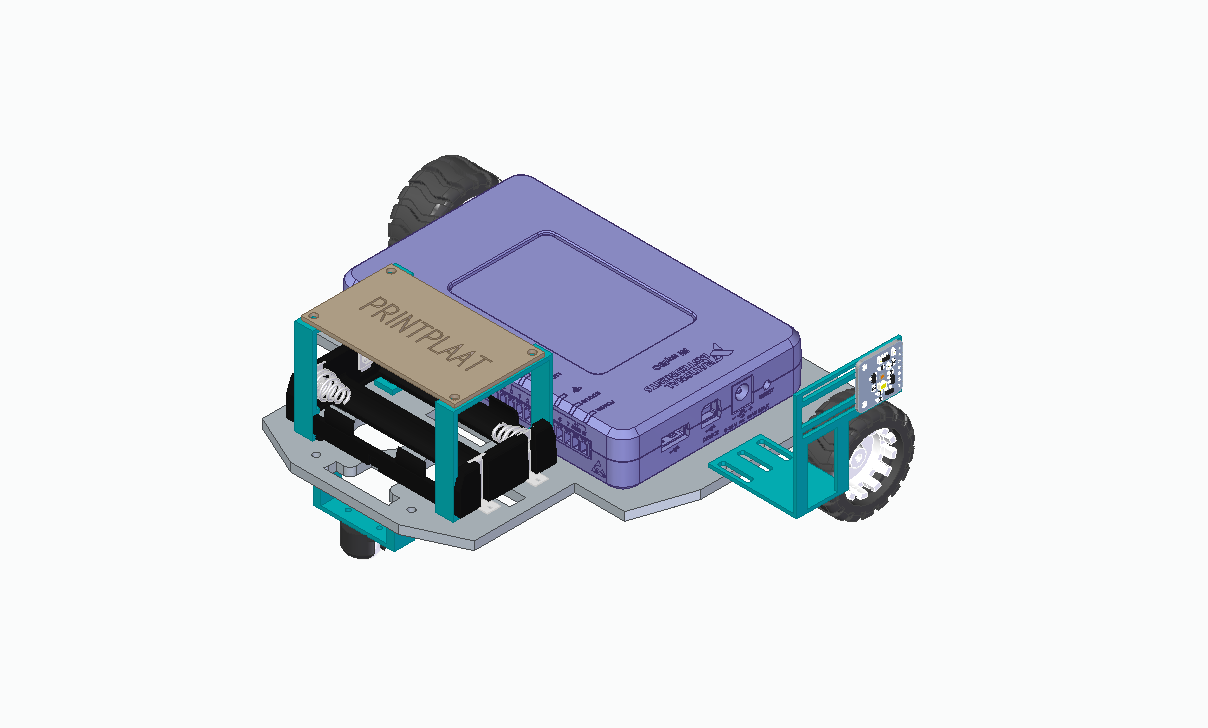
\includegraphics[width=\textwidth]{FotoChassisVerslag (1)}
		\caption{CAD model}
		\label{fig:chassis1}
	\end{figure}
	\begin{figure}[h]
	\centering
	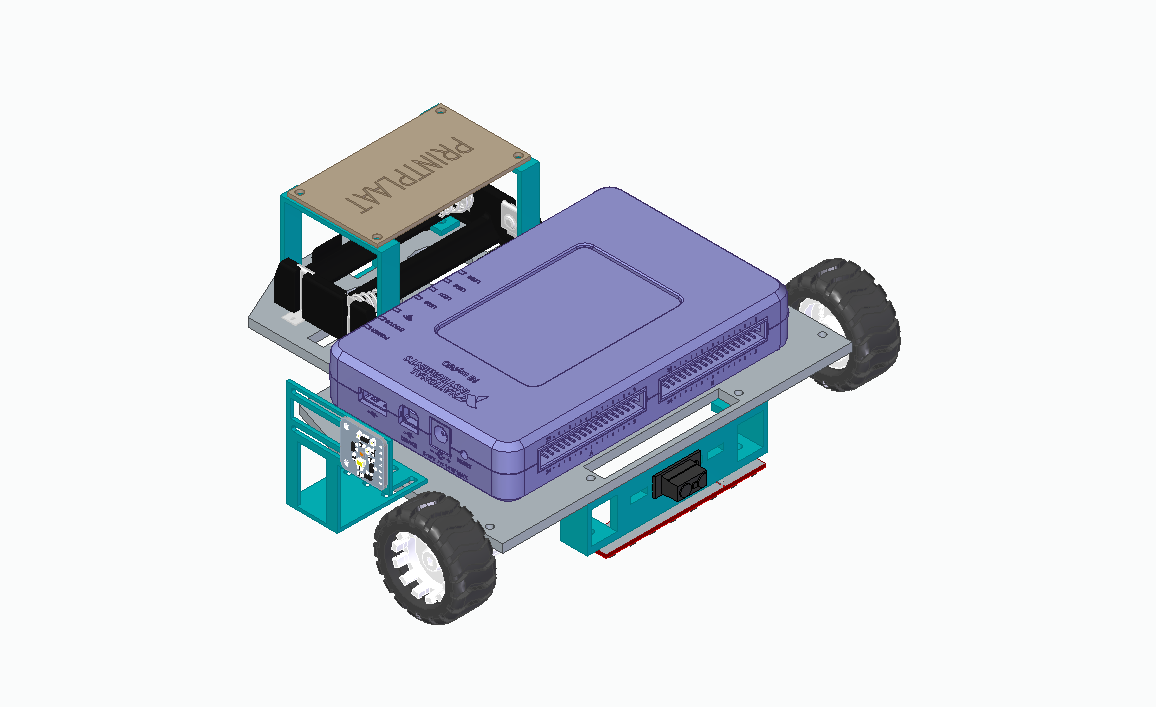
\includegraphics[width=\textwidth]{FotoChassisVerslag (2)}
	\caption{CAD model}
	\label{fig:chassis2}
	\end{figure}
	\clearpage
		
	\section{Implementatie in Labview}
	Aangezien de NI MyRio onze microcontroller is, moesten we al onze onderdelen in LABVIEW programmeren. Hieronder wordt er meer uitleg gegeven over de verschillende onderdelen, namelijk de reflectiesensor, de kleursensor, de afstandssensor en de motoren.
	% Momenteel zijn we nog vollop bezig met het implementeren van de code voor de verschillende onderdelen en commando's in LABVIEW. We hebben ondertussen wel al de lijnsensor grotendeels geïmplementeerd, waar verder nog uitleg over wordt gegeven.
		\subsection{Reflectiesensor}
		De lijnsensor geeft als input een array van 8 analoge spanningen tussen 0V en 5V. Deze moet worden omgezet naar een array met 8 waarden die ofwel 0 ofwel 1 zijn. 0 wil zeggen dat de sensor de lijn niet detecteert en komt overeen met een inputwaarde tussen 0V en 3.3V. Daarnaast kan de sensor bij 1 wel de lijn zien en dit komt overeen met een inputwaarde tussen 3.3V en 5V. Eenmaal de nieuwe array is bepaald, moet deze worden omgezet naar besturing van de wagen. 
		
		
		De waarden worden nu één voor één gecontroleerd op een 1 of een 0, maar er wordt ook telkens bijgehouden op welke index van de array we zitten. Er gebeurt niks tot er bij een specifieke index een 1 wordt gezien. Dan wordt namelijk een waarde tussen -7 en 7 overgebracht naar de volgende lus. Afhankelijk van hoever naar buiten de 1 staat (in de array), zal de doorgegeven waarde groter of kleiner zijn. Zo zal de waarde bijvoorbeeld 7 zijn als de eerste index al een 1 bevat en -7 wanneer bij elke index van de array de waarde 0 is behalve bij de laatste. De mogelijke waarden zijn ±7, ±5, ±3, ±1. Nadat er voor de eerste keer een 1 is aangetroffen, zal telkens wanneer opnieuw een 1 wordt tegengekomen, één eenheid worden afgetrokken van de waarde die tot dan toe werd bekomen. Dit wijst erop dat het wagentje minder aan de buitenkant (ten opzichte van de lijn) zit bij een positief getal, of juist meer naar buiten zit bij een negatief getal. Op die manier kan een onderscheid gemaakt worden van hoe ver (grootte van het getal) het wagentje relatief van de lijn is verwijderd en langs welke kant (positief of negatief getal). Wanneer het wagentje perfect op de lijn rijdt, zullen de 4de en 5de index van de array een 1 bevatten en zal de bepaalde waarde nul zijn, wat wil zeggen dat het wagentje niets moet doen. Aan de hand van de twee ingevoerde waarden die zorgen voor de snelheid van de twee wielen kan het wagentje dan naar een bepaalde kant draaien met een bepaalde scherpte. Hoe groter het getal, hoe scherper de draai naar binnen zal zijn.
		
		Daarnaast kan het ook zijn dat de array alleen enen bevat. Dit wil zeggen dat het wagentje op de stopstreep staat (want alle acht sensoren detecteren de lijn). Hiervoor is een apart geval nodig die eerst controleert of alle elementen in de array 1 zijn. Als dit het geval is, zal het wagentje onmiddellijk stoppen. Zo niet dan zal de wagen worden bijgestuurd via de berekende waarde. Dit is nodig omdat bij een array van alleen maar 1’en de berekende waarde gelijk is aan nul (7-7x1) net zoals wanneer het wagentje perfect op de lijn rijdt. Bijgevolg zal het wagentje dan niks doen.
		%De analoge reflectiesensor moet geprogrammeerd worden zodat het een lijn kan volgen. Dit kan met behulp van acht sensoren. We hebben het zo geprogrammeerd dat we alle sensoren van buiten naar binnen overlopen om te kijken of de sensor een lijn al dan niet detecteerd. Vanaf dat een sensor de lijn ziet, zal het een numerieke waarde geven. Hoe meer de sensor naar binnen ligt, hoe kleiner deze waarde zal zijn. Dit wil namelijk zeggen dat de wagen minder op de rand van de lijn aan het rijden is. Als de sensor over het midden begint waar te nemen, zal het cijfer echter negatief worden. Op die manier krijgen we een indicatie van de kant waar de wagen rijdt en hoe sterk hij van het midden afwijkt. Op die manier kunnen we de wagen dan bijsturen, namelijk hoe verder van de lijn, hoe positiever/negatiever de waarde en hoe meer de wagen bijgestuurd moet worden. Bij het herkennen van de stoplijn zullen alle acht sensoren de streep detecteren en zullen we zo de wagen kunnen bijsturen tot stoppen.
		
		\subsection{Kleursensor}
		Via de input van de kleursensor kunnen we bepalen welke kleur het licht uitschijnt. Als de waarde van de weerstand rond 1000 Ohm zit, detecteert de sensor rood, indien de waarde rond 560 Ohm zit, detecteert de sensor groen licht. Bij rood licht zal de wagen blijven wachten tot het licht op groen springt. Zolang de sensor rood aanduidt, zal de input steeds opnieuw worden gecontroleerd. Vanaf het licht groen wordt, zal het wagentje vertrekken door de waarden voor de motor niet meer op nul te zetten, maar op een hoger voltage.
		
		
		%Als de waarde tussen … zit, detecteert de sensor rood, indien de waarde tussen … zit, detecteert de wagen groen licht.
		\subsection{Afstandssensor}
		Deze sensor detecteert objecten tussen 2cm en 10cm. Als een object zich dichter dan 10 cm (en verder dan 2cm) bevindt, stopt de wagen onmiddellijk. Dit wil zeggen dat de waarden van de motor op dit moment 0 volt zijn.
		%De afstandssensor zullen we zo moeten implementeren dat het een obstakel dat dichter is dan 10 cm kan detecteren, om te kunnen stoppen en een botsing te vermijden.  
		
		\subsection{Motoren}
		De motoren zullen we individueel moeten kunnen aansturen, zodat we het wagentje  kunnen bijsturen indien het niet recht rijdt of een bocht moet maken. We zullen dit doen door eerst en vooral de positie van het wagentje te bepalen. Dan zullen we de snelheid met behulp van de frequentie instellen, de output dan weergeven en daarna de nieuwe richting weer instellen via de input, gegeven door de lijnsensor. 

		
	%\section{Bereikte resultaten}
	
	\section{Toekomstige doelen}
	(wat er nog verbeterd kan worden - met planning voor extra berekeningen)
	\subsection{Planning} % anders noemen eerder we zouden nog dan en dan dat doen
	(welke stappen zouden we nog ondernemen (indien meer tijd) om ons resultaat te verbeteren)
	
	
	\section{Planning}
	\begin{tabular}{lll}
		& Taak & Datum \\ \hline
		1 & Code & \\
		1.1 & Richting kiezen & \\
		1.1.1 & Motoren aansturen & \\
		1.2 & Lijndetectie & 25/03 \\
		1.2.1 & Reflectie sensor inlezen & 25/03\\
		1.2.2 & Reflectie sensor interpreteren & 25/03 \\
		1.3 & Obstakels detecteren & \\
		1.3.1 & Afstandssensor inlezen & \\
		1.3.2 & Afstandssensor interpreteren & \\
		1.4 & Lichten herkennen & \\
		1.4.1 & Kleursensor inlezen & \\
		1.4.2 & Kleursensor interpreteren & \\
		1.5 & Stoplijn herkennen & 25/03\\
		1.5.1 & Reflectiesensor inlezen & 25/03\\
		1.5.2 & Reflectiesensor interpreteren & 25/03\\
		1.6 & Interface maken & \\
		1.6.1 & Vizualisatie Labview & \\
		\hline
		2 & Bouw & \\
		2.1 & CAD model & 25/03\\
		2.1.1 & Wiel & 25/03\\
		2.1.2 & Schroef & \\
		2.1.3 & Kleursensor & \\
		2.1.4 & Afstandssensor & \\
		2.1.5 & Reflectiesensor & \\
		2.1.6 & Chassis & 25/03\\
		2.1.7 & Bevestigingsbeugel motor & \\
		2.1.8 & Microcontroller & \\
		2.1.9 & Printplaat & \\
		2.2 & Chassis printen & \\
		2.3 & Model schetsen & 11/03\\
		2.4 & Technische tekeningen & 01/04\\
		2.5 & Onderdelenlijst & 11/03\\
		2.6 & Berekeningen & \\
		2.6.1 & Draaicirkel & \\
		2.7 & Wagentje maken & \\
		\hline
		3 & Prensentatie & \\
		3.1 & Tussentijds verslag & 01/04 \\
		3.2 & Tussentijdse presentatie & 01/04\\
		3.3 & Eindeverslag & 27/05 \\
		3.4 & Eindpresentatie & 27/05\\ \hline
	\end{tabular}


	
	\chapter{Bijlagen}
	
	\section{Financieel Rapport}
			\begin{tabular}{  l | l | l | l | l }
			
			& Product & Aantal & Prijs per stuk & Totaal  \\ \hline
			1 & Bieding & & & 1400 \\ \hline
			2 & Wiel 42x19mm & 2 & 35.00 & 70 \\ \hline
			3 & Ball Caster & 1 & 60.00 & 60   \\ \hline
			4 & TCS34725 Kleur sensor BOB  & 1 & 150.00 & 150   \\ \hline
			5 & QTR-8A analoge reflectie sensor array & 1 & 150.00 & 150 \\ \hline
			6 & JST Connector 2p 2mm M haaks & 1 & 5.00 & 5 \\ \hline	
			7 & Micro metal gear motor beugel & 2 & 25.00 & 50 \\ \hline
			8 & Breadboard Full-size & 1 & 105.00 & 105   \\ \hline
			9 & NI MyRio & 1 & 240.00 & 240 \\ \hline
			10 & Optische Afstandssensor (digitaal) & 1 & 160.00 & 160  \\ \hline
			11 & Oplaadbare LITHIUM-ION & 4 & 90 & 360 \\ \hline
			12 & Motorschield IC & 1 & 70 & 70  \\ \hline
			13 & Male headers 10 & 4 & 5 & 20   \\ \hline
			14 & Micro Metal Gear Motor 100:1 & 2 & 160.00 & 320 \\ \hline
			15 & Chassis & 1 & & \\ \hline
			16 & Printplaat & & &  \\ \hline
			& Totaal Bedrag & & & 3500\\ 
			& Bedrag Uitgegeven & & & 3160 \\ 
			& Overige Bedrag & & & 340
			
		\end{tabular}
		
	%	\subfile{circuit}
	\section{elektronisch circuit}
	% elektronische circuit -> verduidelijkt verbinding microcotrollers, sensoren en actuatoren 
	\section{Bronnenlijst}
	
	\section*{Besluit}
	Wat is gelukt, wat niet, wat kunnen we nog verbeteren in de toekomst, moeilijkheden, tevreden?
\end{document}